\documentclass[12pt]{article}

\usepackage{sbc-template}

\usepackage{graphicx,url}

\usepackage[brazil]{babel}   
%\usepackage[latin1]{inputenc}  
\usepackage[utf8]{inputenc}  
% UTF-8 encoding is recommended by ShareLaTex

\usepackage{amsmath,amssymb}
%\tracingall
\def\horizlist#1#2{%
  \setcounter{enumi}{0}%
  %#3%
  \flushleft
  \dimen0 \linewidth
  \divide\dimen0 by #1\relax
  \advance\dimen0 -#2\relax
  \def\item{\hfil\egroup\penalty50 \hfill
  \refstepcounter{enumi}%
  \leavevmode\hbox to \dimen0 \bgroup\space(\theenumi)\space}%
  \leavevmode\bgroup\hskip 0pt plus -1fill }

\def\endhorizlist{\hfil\egroup\endflushleft}

\sloppy

\title{Trabalho Aula 7}

\author{Matheus S. Redecker\inst{1}, Thomas Vieira\inst{1}}

\address{Pont\'ificia Universidade Cat\'olica Rio Grande do Sul (PUCRS), \\ Avenida Ipiranga, 6681. Pr\'{e}dio 32, CEP 90619-900. Porto Alegre, RS-Brasil 
  \email{thvieira.rs@gmail.com, matheus.redecker@acad.pucrs.br}
}

\begin{document} 

\maketitle


\section{Descrição do experimento e modelagem}

Um carro é um produto da industria automotiva. Um carro é usado para o transporte, e possui alguns componentes para atingir essa tarefa, alguns componentes são: Motor, sistema de freio, caixa de cambio, injeção eletrônica, painel multimídia, entre outros. Para unificar todos os componentes necessários para um carro funcionar, é utilizado uma serie de micro controladores. O intuito deste trabalho é realizar a modelagem do escalonamento de um carro, através da ferramenta Cheddar, que é uma ferramenta de simulação de escalonamento em tempo real.

Para modelar o carro iremos utilizar 6 processadores, que utilizam o escalonamento Rate Monotonic (RM) \textit{preemptivo}, com os espaços de endereçamentos vazios (a utilidade de cada processador é descrita na próxima seção). Para representar as tarefas realizadas por cada processador  serão criadas 31 tarefas (abreviando para tx, sendo x o número da tarefa). Na maioria dos sistemas os componentes não são isolados um dos outros, por isso é preciso utilizar mensagens para realizar uma comunicação entre componentes. A nossa modelagem contém 12 mensagens, mas com o intuito de reduzir a complexidade na descrição, as mensagens são representadas como tarefas, apenas para simular o comportamento de uma mensagem, mas sem a troca de informações. 

\section{Escalonamento e descrição dos processadores}

Nesta seção iremos apresentar uma amostra do escalonamento de cada processador e a descrição de cada um.

\subsection{Processador 1}

O processador 1 é chamado de \textit{Node 1}. Este processador é responsável pelo controle do motor. Nele são feitas as tarefas t1, t2, t3, t4, t5, t6, e t7. E são transmitidas as mensagens m1, m3, e m10. 
A ordem do escalonamento amostrada na Figura~\ref{node1} é a seguinte:

\begin{enumerate}
    \begin{horizlist}{4}{1cm}
    \item t3
    \item m10
    \item t6
    \item t7
    \item t2
    \item m3
    \item t4
    \item t5
    \item t1
    \item m1
    \end{horizlist}
\end{enumerate}

\newpage{}

\begin{figure}[ht]
	\centering
	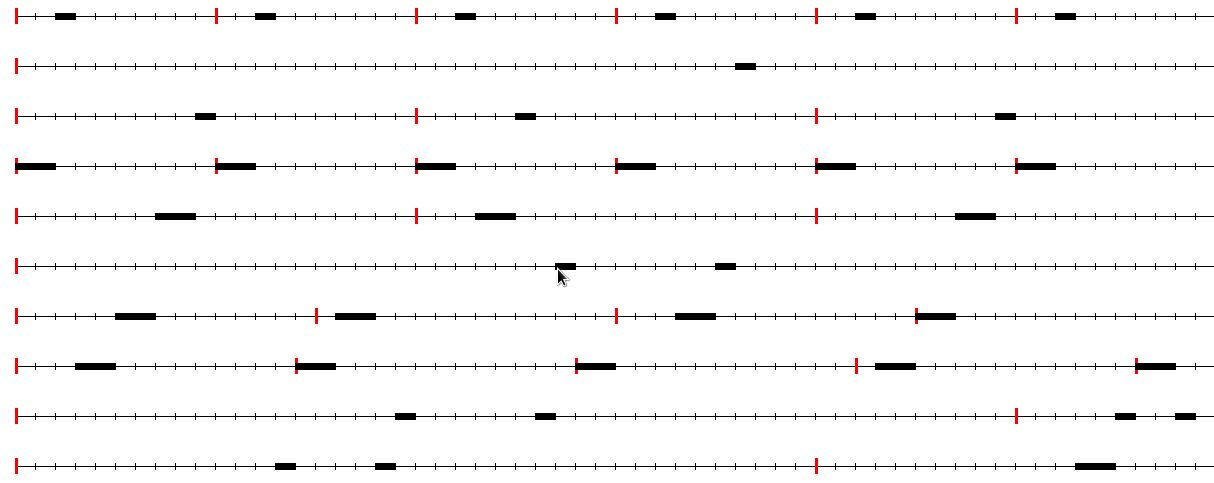
\includegraphics[width=1\textwidth]{node1.jpg}
    \caption{Escalonamento do \textit{Node 1}}
	\label{node1}
\end{figure}

\subsection{Processador 2}
O processador 2 é chamado de \textit{Node 2}. Este processador é responsável pelo controle da caixa de marchas automática. Neste processador são feitas as tarefas t8, t9, t10, e t11. E são transmitidas as mensagens m4 e m11. 
A ordem do escalonamento amostrada na Figura~\ref{node2} é a seguinte:

\begin{enumerate}
    \begin{horizlist}{3}{1cm}
    \item t9
    \item t10
    \item m11
    \item t8
    \item m4
    \item t11
    \end{horizlist}
\end{enumerate}

\begin{figure}[ht]
	\centering
	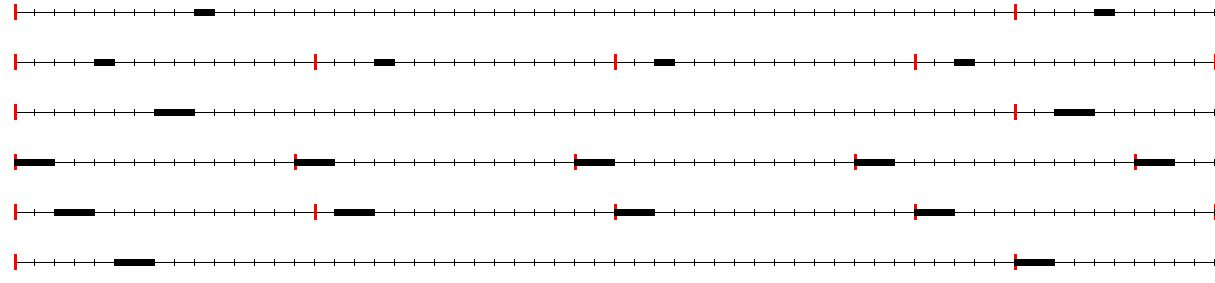
\includegraphics[width=1\textwidth]{node2.jpg}
    \caption{Escalonamento do \textit{Node 2}}
	\label{node2}
\end{figure}

\subsection{Processador 3}

O processador 3 é chamado de \textit{Node 3}. Este processador é responsável pelo anti bloqueio do sistema de freio e pelo controle dinâmico do veículo. Neste processador são feitas as tarefas t12, t13, t14, t15, t16, e t17. E são transmitidas as mensagens m5, m6, m7, e m12. 
A ordem do escalonamento amostrada na Figura~\ref{node3} é a seguinte:

\begin{enumerate}
    \begin{horizlist}{4}{1cm}
    \item m12
    \item m5
    \item m6
    \item m7
    \item t12
    \item t13
    \item t14
    \item t15
    \item t16
    \item t17
    \end{horizlist}
\end{enumerate}

\newpage{}

\begin{figure}[ht]
	\centering
	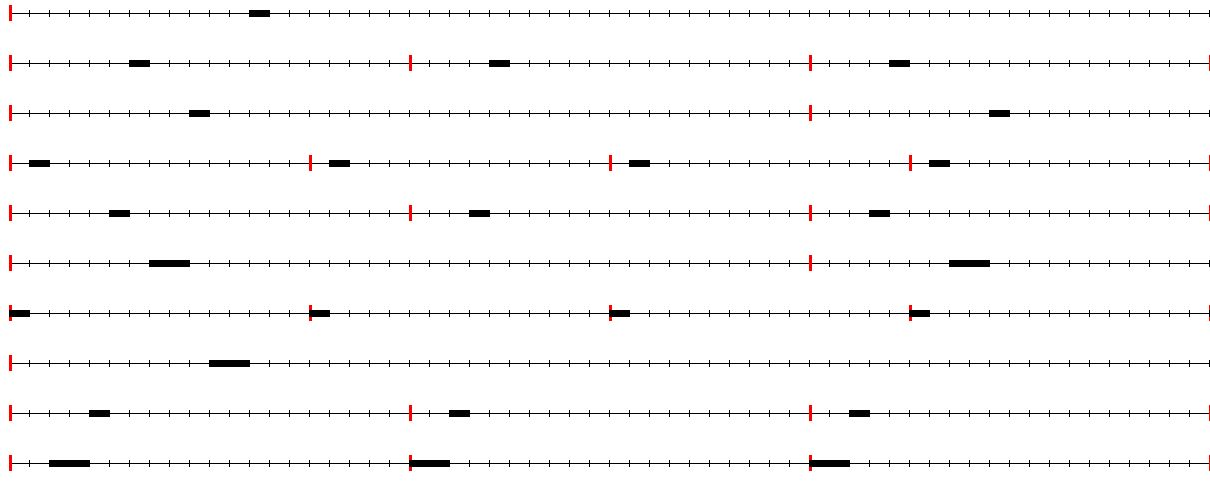
\includegraphics[width=1\textwidth]{node3.jpg}
    \caption{Escalonamento do \textit{Node 3}}
	\label{node3}
\end{figure}

\subsection{Processador 4}

O processador 4 é chamado de \textit{Node 4}. Este processador é responsável pelo controle do sensor do ângulo de roda e pelo corretor de farol dinâmico. Neste processador são feitas as tarefas t18 e t19. E é transmitida a mensagem m2. 
A ordem do escalonamento amostrada na Figura~\ref{node4} é a seguinte:

\begin{enumerate}
    \begin{horizlist}{3}{1cm}
    \item m2
    \item t18
    \item t19
    \end{horizlist}
\end{enumerate}

\begin{figure}[ht]
	\centering
	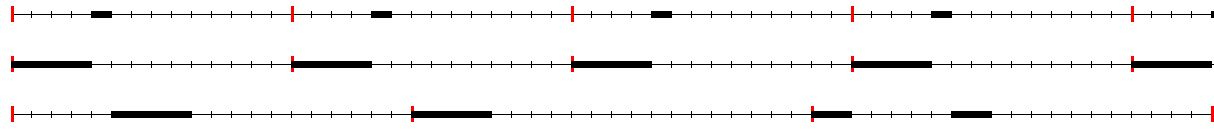
\includegraphics[width=1\textwidth]{node4.jpg}
    \caption{Escalonamento do \textit{Node 4}}
	\label{node4}
\end{figure}

\subsection{Processador 5}

O processador 5 é chamado de \textit{Node 5}. Este processador é responsável pelo controle da suspensão. Neste processador são feitas as tarefas t20, t21, t22, t23, e t24. E é transmitida a mensagem m9. 
A ordem do escalonamento amostrada na Figura~\ref{node5} é a seguinte:

\begin{enumerate}
    \begin{horizlist}{3}{1cm}
    \item m9
    \item t20
    \item t21
    \item t22
    \item t23
    \item t24
    \end{horizlist}
\end{enumerate}

\begin{figure}[ht]
	\centering
	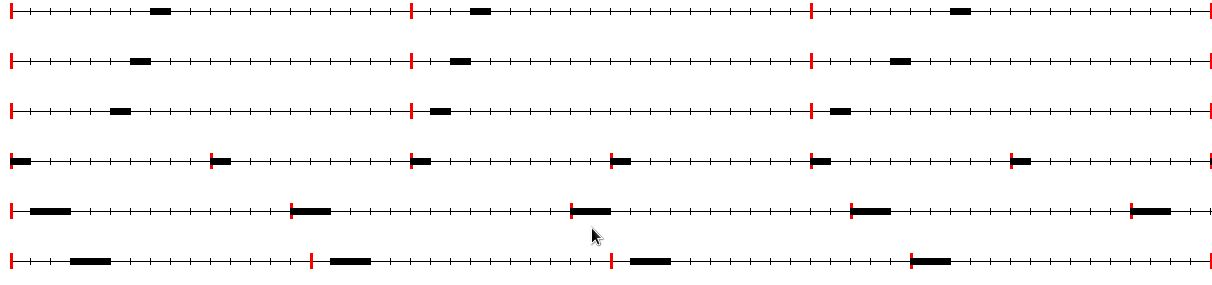
\includegraphics[width=1\textwidth]{node5.jpg}
    \caption{Escalonamento do \textit{Node 5}}
	\label{node5}
\end{figure}

\subsection{Processador 6}

O processador 6 é chamado de \textit{Node 6}. Este processador é responsável pelo controle da suspensão. Neste processador são feitas as tarefas t25, t26, t27, t28, t29, t30, e t31. E é transmitida a mensagem m8. 
A ordem do escalonamento amostrada na Figura~\ref{node6} é a seguinte:

\begin{enumerate}
    \begin{horizlist}{3}{1cm}
    \item m8
    \item t25
    \item t26
    \item t27
    \item t28
    \item t29
    \item t30
    \item t31
    \end{horizlist}
\end{enumerate}

\begin{figure}[ht]
	\centering
	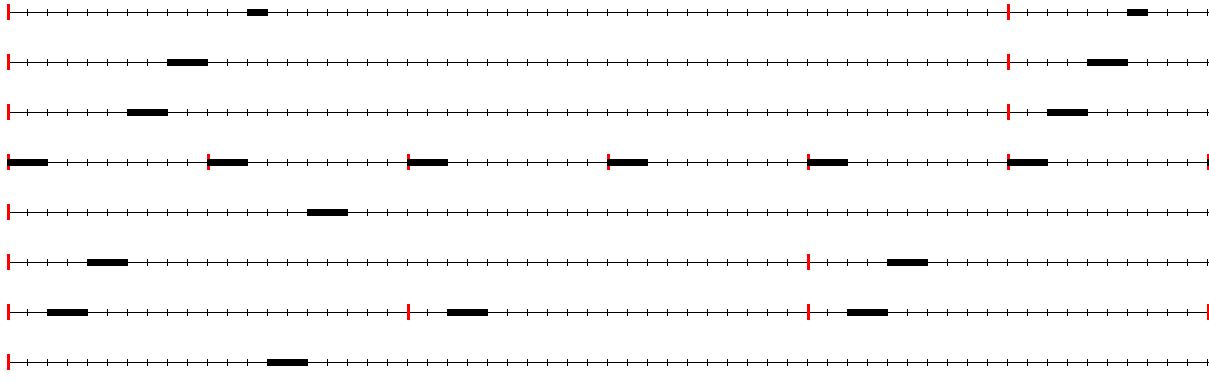
\includegraphics[width=1\textwidth]{node6.jpg}
    \caption{Escalonamento do Node 6}
	\label{node6}
\end{figure}

\section{Tabela}

A Tabela~\ref{tab} contém os valores de utilização (U), o \textit{upper bound}, e o período de escalonamento para o conjunto em cada processador. Como as mensagens foram modeladas como tarefas, no calculo do \textit{upper bound}, as mensagens foram incluídas no calculo e consequentemente no número de tarefas.

\begin{table}[ht]
\centering
\caption{Tabela com os parâmetros para cada processador}
\label{tab}
\begin{tabular}{|c|c|c|c|}
\hline
\textbf{Node} & \textbf{U(\%)} & \textbf{Upper bound} & \textbf{H(ms)} \\ \hline
1             & 0,84619    &      0,71773         & 4200           \\ \hline
2             & 0,44286    &      0,73477         & 1050           \\ \hline
3             & 0,48833    &      0,71773         & 600            \\ \hline
4             & 0,55714    &      0,77976         & 140            \\ \hline
5             & 0,52619    &      0,73477         & 420            \\ \hline
6             & 0,49000    &      0,72406         & 200            \\ \hline
\end{tabular}
\end{table}

\section{Resultados e modificações}

O sistema é escalonável, pois todas os processadores conseguem escalonar suas tarefas. Excluindo o \textit{Node 1}, todos os outros processadores são confirmados escalonáveis pela \textit{upper bound}. O \textit{upper bound} consistem em analisar se o sistema é escalonável, se a soma da utilização de todas as tarefas ($\sum{U_{i}}$) são menores que $n (2^{\frac{1}{n}} - 1)$. Mas essa regra não prova que o sistema não é escalonável, apenas se ele é, caso satisfaça a formula. Com isso, através dos experimentos foi possível mostrar que o \textit{Node 1} é escalonável.

\end{document}


